\documentclass[12pt]{beamer}
\usepackage[utf8]{inputenc}
\usepackage[czech]{babel}
\usepackage[IL2]{fontenc}
\usepackage{lmodern}
\usepackage{graphicx}
\usepackage{epstopdf}

\mode<presentation> {
  \usetheme{Berlin}
  \setbeamercovered{transparent}
}

\title{Implementace imperativního jazyka IFJ14}
\author{Tým 113}
\institute{Fakulta informačních technologií \\Vysokého učení technického v~Brně}
\date{\today}

\begin{document}

\begin{frame}
	\titlepage
\end{frame}

\begin{frame}
	\frametitle{IFJ14}
	\framesubtitle{Tým 113 -- složení}
	Vedoucí týmu: Antonín Marko
	\begin{itemize}
		\item \textbf{Lexikální analyzátor:} Tomáš Pružina a Martin Juřík
		\item \textbf{Syntaktický a sémantický analyzátor:} Antonín Marko
		\item \textbf{Interpret:} Tomáš Pružina
		\item \textbf{Algoritmy předmětu IAL:} Petr David a Martin Juřík
		\item \textbf{LL-gramatika a testování:} Martin Kubíček
	\end{itemize}
\end{frame}

\begin{frame}
	\frametitle{Lexikální analyzátor}
	\framesubtitle{Schéma konečného automatu}
	\begin{figure}
		\centering
			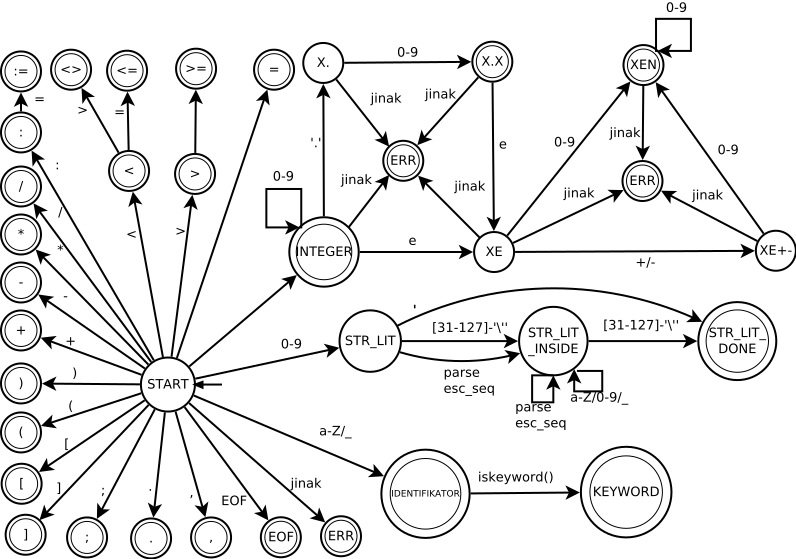
\includegraphics[width=0.7\textwidth]{KA-scanner.png}
	\end{figure}
\end{frame}

\begin{frame}
	\frametitle{Syntaktický a semantický analyzátor}
	\begin{itemize}
		\item Analýza shora dolů
		\item Kontrola datových typů
		\item Načítání podle LL-tabulky
		\item Vnitřní kód řešen Abstraktním syntaktickým stromem
		\item Výrazy řešeny Shunting-yard algoritmem
	\end{itemize}
\end{frame}

\begin{frame}
	\frametitle{Syntaktický a semantický analyzátor}
	\framesubtitle{Příklad AST}
	\begin{figure}
		\centering
			\includegraphics[width=0.6\textwidth]{ast.png}
	\end{figure}	
\end{frame}

\begin{frame}
	\frametitle{Shunting-yard algoritmus}
	\framesubtitle{Přímé generování AST}
	\begin{itemize}
		\item Metoda zpracování výrazů
		\item Převod infixového zápisu do postfixového
		\item \textbf{Modifikace:} Přímé generování AST
		\begin{itemize}
			\item Pouze jediný průchod
		\end{itemize}
		\item Př.: \texttt{ 3 + 4 $\Rightarrow$ 3 4 + }
		\begin{figure}
			\centering
				\includegraphics[width=0.3\textwidth]{sya.png}
		\end{figure}
	\end{itemize}
\end{frame}

\begin{frame}
	\frametitle{Interpret}
	\begin{itemize}
		\item Interpretuje AST
		\item Pracuje s tabulkou symbolů
		\item Kontrolování platných operací
		\begin{itemize}
			\item Neinicializované proměnné
			\item Dělení nulou
		\end{itemize}
	\end{itemize}
\end{frame}

\begin{frame}
	\frametitle{Algoritmy do předmětu IAL}
	\framesubtitle{Funkce \texttt{sort}}
	{\Large QuickSort}
	\begin{itemize}
		\item Složitost: $n*log(n)$
		\item Nestabilní algoritmus
		\item Problém volby pivotu
	\end{itemize}
\end{frame}

\begin{frame}
	\frametitle{Algoritmy do předmětu IAL}
	\framesubtitle{Funkce \texttt{find}}
	{\Large Knuth-Morris-Prattův algoritmus}
	\begin{itemize}
		\item Slouží na vyhledávání podřetězců v řetězcích
		\item Konečný automat využívající hrany ANO/NE
		\item Pole FAIL uchovávající hodnoty posunů zpět
		\item Nevýhodou KMP je, že z každého uzlu vychází tolik hran, kolik je znaků abecedy
	\end{itemize}
\end{frame}

\begin{frame}
	\frametitle{Implementovaná rozšíření}
	\framesubtitle{\texttt{ARRAY, FOR, REPEAT, BOOLOP, ELSEIF}}
	\texttt{ARRAY}
	\begin{itemize}
		\item Implementované v tabulce symbolů
	\end{itemize}
	\texttt{FOR} cyklus
	\begin{itemize}
		\item Doplnění pravidel do LL-tabulky
	\end{itemize}
	\texttt{REPEAT} cyklus
	\begin{itemize}
		\item Podobný postup analýzy jako u cyklu \texttt{while}
	\end{itemize}
	\texttt{BOOLOP}
	\begin{itemize}
		\item Doplněné operátory do Shunting-yard algoritmu
	\end{itemize}
	\texttt{ELSEIF}
	\begin{itemize}
		\item Podpora vynechání klíčového slova \texttt{else}
	\end{itemize}
\end{frame}

\begin{frame}
	\frametitle{Jednoduchý příklad}
	\begin{figure}
		\centering
			\includegraphics[width=0.8\textwidth]{program.png}
	\end{figure}
\end{frame}

\end{document}
